\section{Задание 1}

В задании при наведении курсора мыши на название животного, в ячейке таблицы появляется рисунок этого животного. При уведении курсора в сторону рисунок исчезает. Фон страницы любой светлый. Цвет текста тёмный, но не чёрный.

\begin{center}
  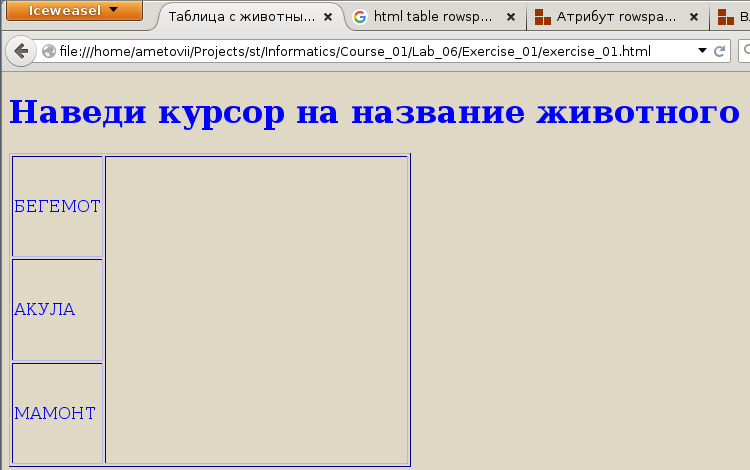
\includegraphics[width=10cm]{img/Exercise_01/01.png}
  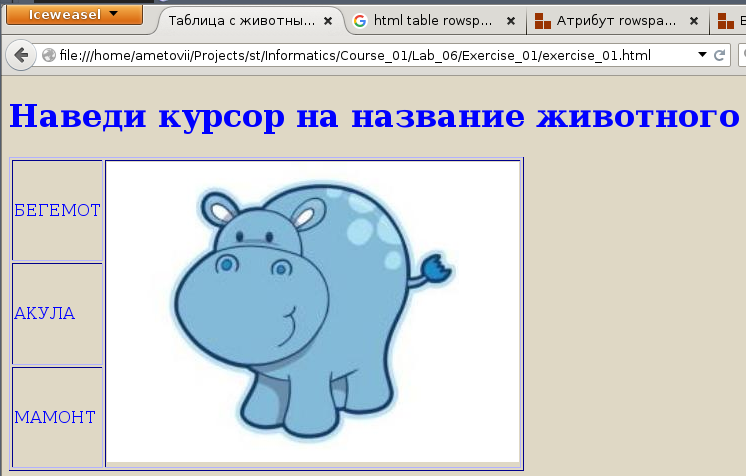
\includegraphics[width=10cm]{img/Exercise_01/02.png}
  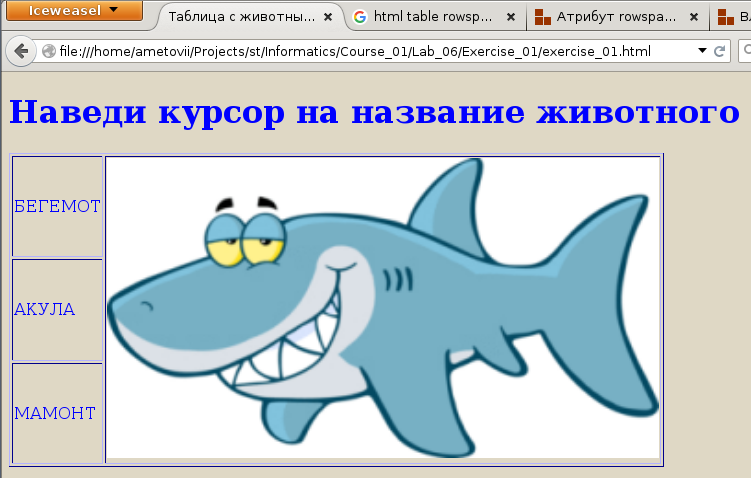
\includegraphics[width=10cm]{img/Exercise_01/03.png}
  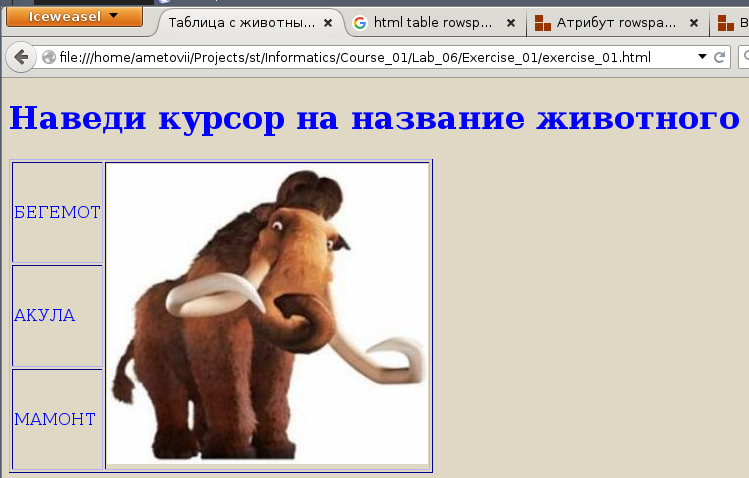
\includegraphics[width=10cm]{img/Exercise_01/04.png}
\end{center}

Исходный код \verb|exercise_01.html|:

\begin{verbatim}
<!doctype html>
<html>
  <head>
    <title>Таблица с животными</title>
    <meta charset='utf-8' />
     <style type="text/css">
      body {background-color:#dfd8c5; color:#0000ff;}
      img {width:274; height:233}
     </style>
     <script>
       function changeImage(imageType){
	   var someImage=document.getElementById('pic');	   
	   if (imageType=='begemot') someImage.src="Images/begemot.jpg";
	   if (imageType=='shark') someImage.src="Images/shark.png";
	   if (imageType=='mamont') someImage.src="Images/mamont.jpg";
       }

       function clearImage(){
	   var someImage=document.getElementById('pic');
	   someImage.src="Images/blank.png";
       }
     </script>
     </head>
  <body>
    <h1>Наведи курсор на название животного</h1>
    <table border="1">
      <tr><td onMouseOver="changeImage('begemot');"
	      onMouseOut="clearImage();">БЕГЕМОТ</td><td rowspan="3">
	  <img name="pic" id='pic' src="Images/blank.png"/></td></tr>
      <tr><td onMouseOver="changeImage('shark');"
	      onMouseOut="clearImage();">АКУЛА</td></tr>
      <tr><td onMouseOver="changeImage('mamont');"
	      onMouseOut="clearImage();">МАМОНТ</td></tr>
    </table>
  </body>
</html>
\end{verbatim}
